\documentclass[10pt,letterpaper]{article}
\usepackage{geometry}
\geometry{margin=1in}
\usepackage{graphicx}

\setlength{\parindent}{0pt}
\setlength{\parskip}{0.5em}

%make lists tighter
\usepackage{enumitem}
\setlist{nolistsep}
\usepackage{float}
%reduce spacing before and after section
\usepackage{titlesec}
% reduce section, subsection, etc spacing
\usepackage{titlesec}
\titlespacing*{\section}{0pt}{0\baselineskip}{0\baselineskip}
\titlespacing*{\subsection}{0pt}{0\baselineskip}{0\baselineskip}
\titlespacing*{\subsubsection}{0pt}{0\baselineskip}{0\baselineskip}

%reduce list spacing
\usepackage{enumitem}
\setlist{nosep}

\usepackage[hidelinks]{hyperref}

\title{Lab 2 - Cloud Data, Stat 214, Spring 2025\vspace{-2em}}

% submission must not contain any of your names
% but feel free to make a version for yourself with your names on it
% \author{Your names}

\begin{document}
\maketitle


\section{Introduction}
In the Arctic, clouds play a crucial role in regulating air temperatures and influencing the region's sensitivity to rising surface air temperatures. To systematically assess whether surface air temperatures depend on increasing atmospheric carbon dioxide levels, accurate measurements of cloud distribution are essential. However, traditional multispectral sensors with a single viewing angle faced significant challenges in cloud detection. This difficulty arises because the optical properties of liquid- and ice-water cloud particles closely resemble those of ice- and snow-covered surfaces.

The launch of the Multiangle Imaging SpectroRadiometer (MISR) in 1999 introduced a significant advancement, providing nine different angular views of each Earth scene across four spectral bands. MISR’s remote sensing observations strongly suggested the potential for distinguishing clouds from snow- and ice-covered surfaces (Diner et al., 1999a). However, MISR’s operational cloud detection algorithms were not specifically designed to identify clouds over bright surfaces in polar regions. Given the constraints of large datasets and extremely limited annotations, performing binary cloud classification posed a substantial statistical challenge at the time.

To address this issue, Yu et al. (2008) developed a novel approach to identify cloud-free surfaces by leveraging the high correlations in brightness among different views of the same scene under unobstructed, cloud-free conditions. Their method introduced three physically meaningful features: (1) the correlation (CORR) of MISR images from different viewing angles, (2) the standard deviation (SD) of MISR’s nadir camera across a scene, and (3) a normalized difference angular index (NDAI), which characterizes changes in scene appearance with varying viewing directions.

In this project, our objective is to enhance classification performance using the same dataset by incorporating recent advancements in feature engineering and classification methods.



\section{EDA}
In this project, we analyzed 164 MISR images, of which 3 are annotated. We began by visualizing the three labeled images and conducted a straightforward reality check. This was confirmed by cross-referencing with the labeled images presented in Yu et al.'s paper. Upon inspection, we observed that a significant number of pixels were unlabeled, which may correspond to areas where experts were uncertain. We will discuss our approach and decisions regarding these unlabeled pixels in the Modeling section.
\begin{figure}[H] 
    \centering
    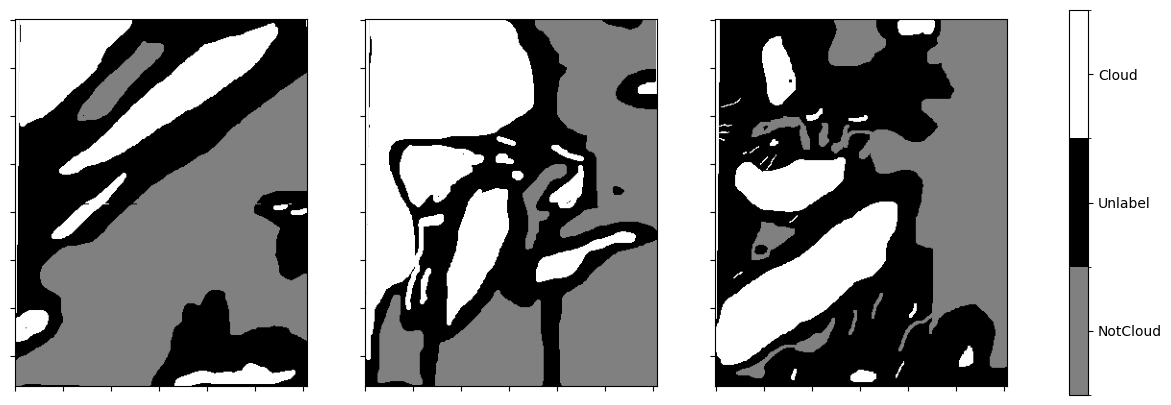
\includegraphics[scale=0.5]{EDA_labeledimg.png}  % Replace with your image file
    \caption{\textbf{Labeled Images O013257, O013490, and O012791}: images labeled by experts. Unlabeled areas may correspond to ambiguous and hard-to-label regions.}
    \label{fig:fig1}
\end{figure}


We also visualized the images captured from different viewing angles. These images exhibited varying overall intensities, with some angles appearing brighter and others darker. Additionally, the intensity contrast between images varied. However, it was challenging to isolate the specific effects of different angles on cloud and non-cloud regions.

To better understand these variations, we quantified the correlations in pixel intensity for cloud and non-cloud regions across different viewing angles. Given the limited sample size (only three labeled images), drawing  conclusions remains challenging. However, we observed that in O012791.npz and O013490.npz, the non-cloud regions exhibited a high correlation in pixel intensity across different angles, whereas O013257.npz appeared to be an outlier.

To validate our findings, we performed a reality check by referring to the existing literature. Yu et al. (2008) noted that a key assumption in this field is that, with MISR, clouds should exhibit greater variations in radiance than other background surfaces, making them easier to detect. Our observations align with this assumption, reinforcing the notion that radiance variability across angles can serve as a useful distinguishing feature for cloud detection.
\begin{figure}[H] 
    \centering
    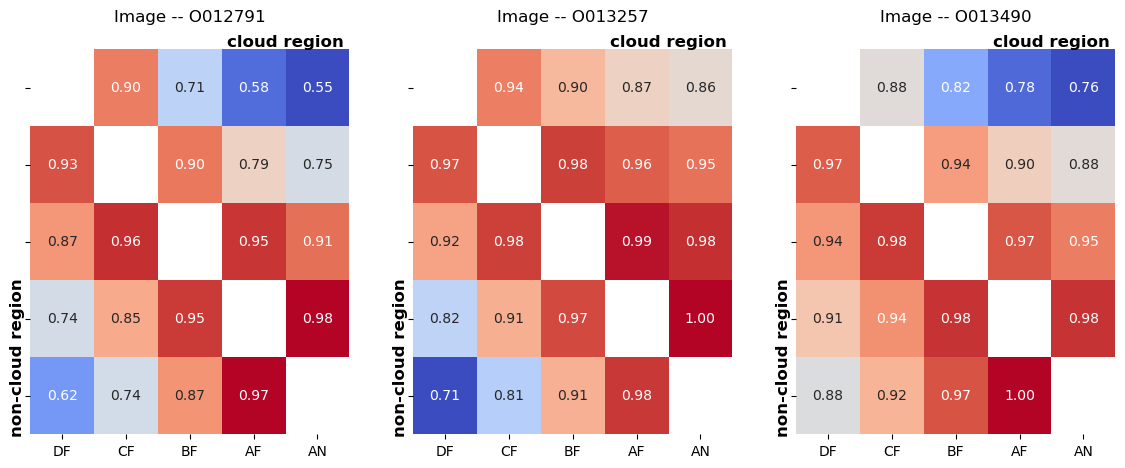
\includegraphics[scale=0.5]{EDA_correlation.png}  % Replace with your image file
    \caption{\textbf{MISR Image Intensity Correlation Across Different Angles:} This heatmap shows the Pearson correlations between different angles. The upper right shows cloud region correlations, and the lower left shows the non-cloud region correlations. 2 out of the 3 labeled images show the trend that non-cloud regions have larger correlations across angels than the cloudy regions.}
    \label{fig:fig2}
\end{figure}


The differences between the two classes (cloud vs. non-cloud) based on the three features—CORR, SD, and NDAI—were visually distinct (see \ref{fig:fig3}). For the CORR feature, pixels labeled as clouds typically exhibited lower values, whereas non-cloud regions had higher values. In the case of SD, non-cloud regions showed lower values, indicating smoother surfaces. For the NDAI feature, non-cloud areas generally had lower values compared to cloud regions. Overall, when combining all three features, the separation between the two classes was visually clear and distinct.
\begin{figure}[H] 
    \centering
    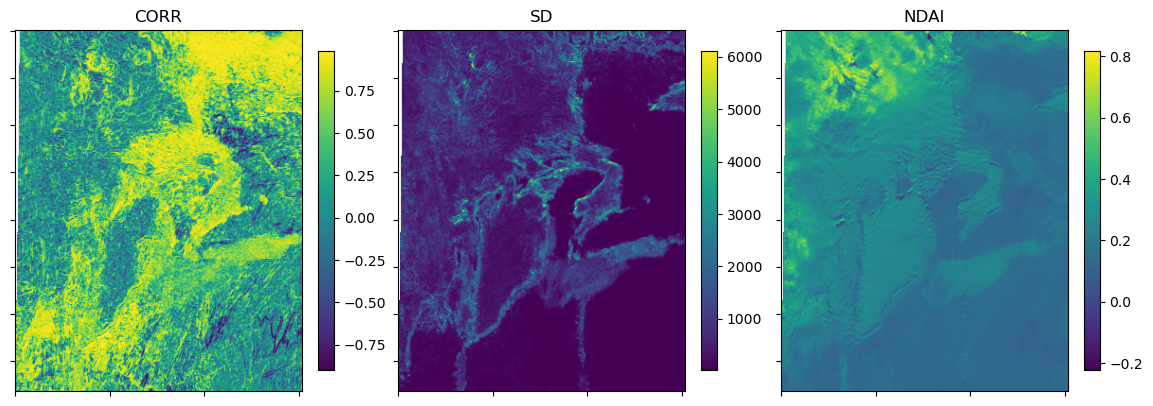
\includegraphics[scale=0.5]{EDA_features.png}  % Replace with your image file
    \caption{\textbf{CORR, SD, NDAI for a representative image O013490}}
    \label{fig:fig3}
\end{figure}

We confirmed these observations quantitatively. All three features demonstrated some degree of separation between the distributions of the two classes. However, no single feature was able to cleanly separate the classes across the three labeled images. For example, in the case of image O013490, the distributions of CORR largely overlapped. In contrast, the SD and NDAI features showed clear separation. This suggests that the three features capture different aspects of the distinction between the two classes, and when used together, they provide valuable information for our downstream classification.
\begin{figure}[H] 
    \centering
    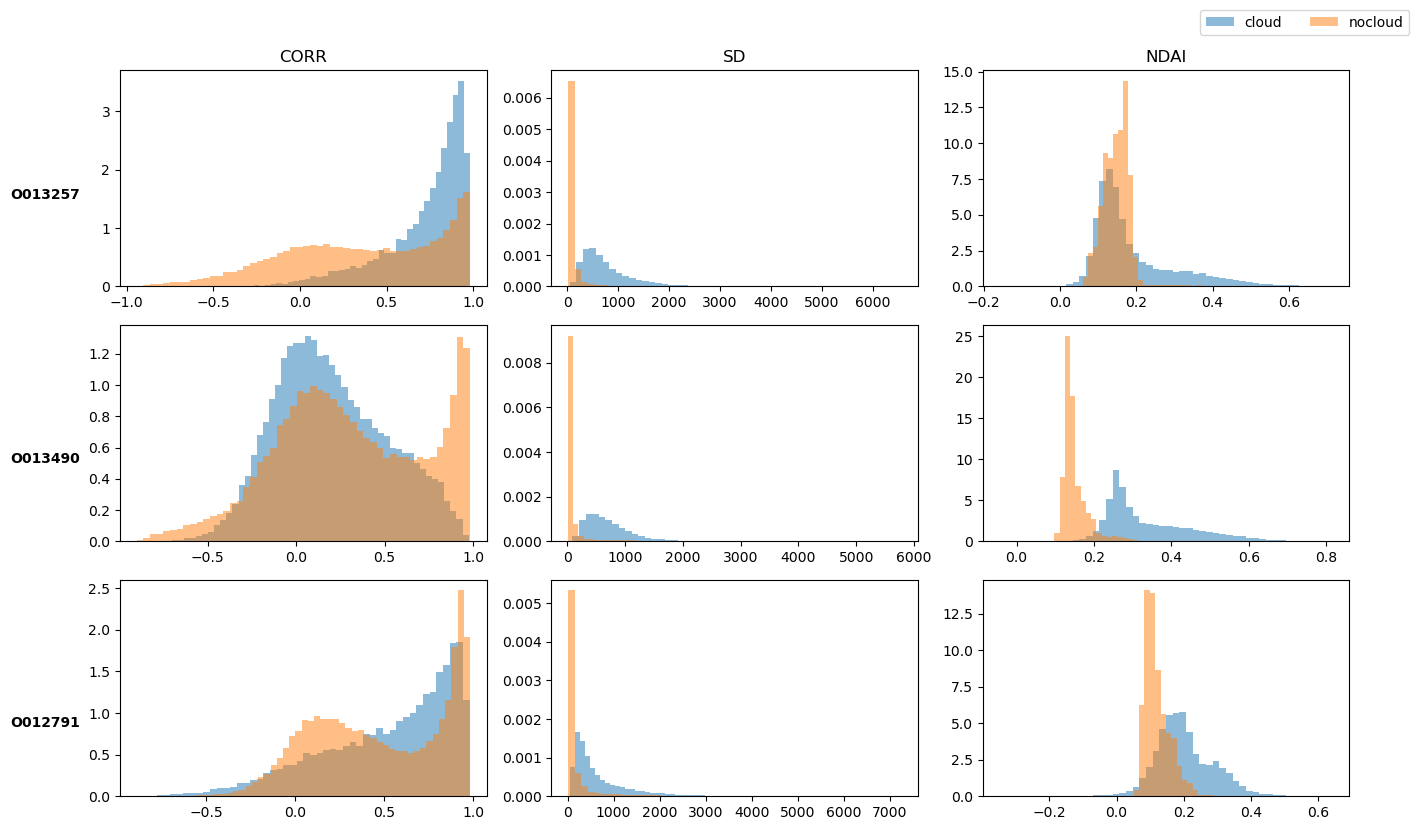
\includegraphics[width=\textwidth]{EDA_dist.png}  % Replace with your image file
    \caption{\textbf{CORR, SD, NDAI distributions for the labeled images}}
    \label{fig:fig3}
\end{figure}

For the unlabeled data, we checked that there are no missing values in this data set. 

\section{Feature Engineering}

In this section, we have analyzed the importance of 8 features using the Random Forest algorithm. We first read three three images with labels, during the reading process we first preprocessed the data, we removed the data points with label 0 that is unlabeled data points. Then the missing values in the feature data X were supplemented with the mean values of the individual columns. Then the target variable y was set as binarized where the data points with clouds were labeled as 1 and those without clouds were labeled as 0. Then we constructed the model using a random forest classifier where we set the number of trees to 100, the drunken inversion depth to 10, and randomly set the number of seeds to 42 to ensure the reproducibility of the results. From the results of Figure 1, the top three feature values are “SD”, “NDAI” and “AN”.
\begin{figure}[H]
    \centering
    \includegraphics[width=1\linewidth]{featureImportance.png}
    \caption{Feature Importance}
    \label{fig:enter-label}
\end{figure}

Based on the results of the previous step, we decided to use the mean of the gradient variation of the values of the three most important features as a new feature variable. The logic of my gradient change calculation is that for each pixel point in the image measure the difference between its value and that of the 8 neighboring pixel points around it and take the average of these differences to represent the intensity of the change in the local area of the changed pixel point at a time. The reason for using gradient variation is that we believe that cloudy and non-cloudy textures are different, and the gradient-mean feature can highlight these local structural differences. In addition, using raw data is susceptible to lighting variations, sensor noise, etc., whereas using gradient operations focuses more on the differences between neighboring pixels, and this local comparison is more stable. In addition, our use of multi-channel gradient averaging can also help us average out some familiar anomalies.

As we can see from the results in Figure 2, our newly created feature values possess high importance.

\begin{figure}[H]
    \centering
    \includegraphics[width=1\linewidth]{newFeature.png}
    \caption{Feature Importance}
    \label{fig:enter-label}
\end{figure}

Next, we utilized transfer learning to improve cloud detection accuracy, allowing us to leverage the unlabeled MISR images before fine-tuning on the more limited, expert-labeled data. We hypothesized that pre-training an autoencoder on the unlabeled dataset would enable the model to learn generalizable patterns of cloud formations and surface characteristics, thus providing additional robust features for us to train our classification models.


We utilized a Lightning-based autoencoder architecture with a sequential encoder-decoder structure. The encoder consists of a flattening operation followed by three linear layers separated by ReLU activation functions. This architecture processes 9×9 pixel patches with eight features, resulting in an input size of 648 dimensions. After extensive experimentation, we determined that an embedding size of eight provided the optimal balance between feature compression and information preservation. This dimensionality was selected based on reconstruction loss curves across various latent space sizes, where we observed diminishing returns with larger embeddings.

After pre-training, we utilized the encoder to transform our labeled training data into the learned embedding space, and its output became input features for our classification models. Our autoencoder's loss function decreased from 60\% to 7\%, demonstrating its improvement at image deconstruction and reconstruction, distilling the images to generalizable patterns. This transfer learning approach improved classification performance compared to models trained solely on the original features, demonstrating the value of leveraging unlabeled data in this domain-specific application.


\section{Modeling}
\subsection{Overview and Data Preparation}
Creating accurate and robust models to distinguish clouds from non-cloud regions is a key objective of our analysis. While the majority (161 of 164) of the images lack labels and cannot be used in a supervised learning setting, the 3 labeled images contain sufficient data points to train classification models that generalize well. Furthermore, although we are only training the models on labeled data, the autoencoder trained on the unlabeled data can be used to generate high-quality representative features which could be potentially capturing the characteristics of the images and predictive to the non-cloud or cloud regions.

We are training our classifiers on a per-pixel basis, having 4 original features as input for each model. As highlighted in Section 3, we selected the 3 most important features (SD, NDAI, CORR) out of the 8 raw features and engineered a new feature by making use of the gradient (grad\_feature). It is worth noting that roughly 30\% of the pixels contain no meaningful label (label = 0), and we dropped all such pixels prior to creating our models. In this way, each sample will contain a valid label either denoting existence of cloud (1) or absence of cloud (-1), eliminating the need to address missing values when training and predicting. The resulting input features compose a matrix with 207681 rows and 4 columns. We also concatenated the latent embeddings generated by autoencoder as predictors. In total, we have 12 features.


We used two of three labeled images as training data and the third as testing. We believe that this split method is mimicking the real life data collection process, where we train on a batch of images, and use our algorithm on newly collected images. All features are standardized to have mean 0 and standard deviation 1 based on the training set, facilitating training for scale-sensitive models such as MLP and SVC.

\subsection{Model 1: Random Forest Classifier}
The Random Forest classifier is an ensemble of decision trees that captures nonlinear relationships, remains robust to outliers and greatly fits classification tasks with a small number of features. All these properties make Random Forest well-suited to our cloud-classification task.

Although Random Forest is relatively insensitive to input distributions, there are 2 assumptions that must be stated and tested before selecting the model. First, a relatively large number of samples is required to prevent underfitting. In our dataset, 150940 samples for training is highly sufficient considering the few features we train the model on. Second, a balanced distribution between outcomes is strongly preferred to avoid majority bias, in which case the model leans towards the majority class and under-predicts the minority class. Our dataset contains 40\% of cloud samples and 60\% of non-cloud samples in the training dataset, making it biased towards the negative class. To address this issue, we applied class weighting to our Random Forest classifier. Class weighting assigns higher importance to minority class samples during training by setting weights inversely proportional to class frequencies. This helps our model penalize misclassifications of the minority class more heavily, effectively reducing bias in predictions. 

We also performed hyperparameter tuning using grid search with cross validation in order to get the best performing model and attenuate overfitting. The parameters that we tuned include max\_depth, min\_samples\_split, max\_features, and n\_estimators.

We evaluated our models by 3 main metrics: classification accuracy on the test set, ROC-AUC on the test set and mean cross-validated accuracy on the training set. The Random Forest model achieves a 83.65\% accuracy and 92.89\% ROC-AUC on the test set, proving its effectiveness in distinguishing cloud pixels from non-cloud ones.  It performed slightly better (85\% precision) on non-cloud pixels, but maintained strong performance (81\% precision) on cloud detection as well, indicating good generalization. Furthermore, the model achieves a 95\% accuracy under 5-fold cross validation, demonstrating its robustness.

\begin{figure}[H]
    \centering
    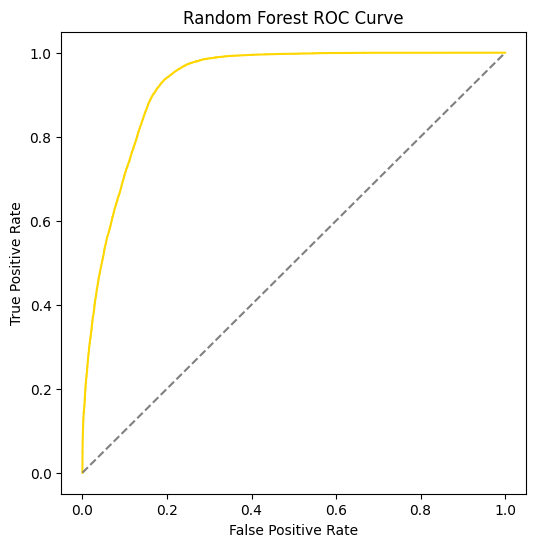
\includegraphics[width=0.5\linewidth]{RF_perf.png}
    \caption{ROC Curve of Random Forest Classifier}
    \label{fig:enter-label}
\end{figure}

\begin{table}[H]
\centering
\caption{Classification Report for Random Forest Classifier}
\begin{tabular}{lcccc}
\textbf{Class} & \textbf{Precision} & \textbf{Recall} & \textbf{F1-Score} & \textbf{Support} \\
-1.0 (Non-Cloud) & 0.85 & 0.88 & 0.87 & 32798 \\
1.0 (Cloud)      & 0.81 & 0.77 & 0.79 & 21244 \\
\textbf{Accuracy} & & & 0.84 & 54042 \\
\textbf{Macro Avg} & 0.83 & 0.82 & 0.83 & 54042 \\
\textbf{Weighted Avg} & 0.84 & 0.84  & 0.84 & 54042 \\
\end{tabular}
\end{table}

\subsection{Model 2: Multi-Layer Perceptron Classifier}
The Multi-Layer Perceptron (MLP) is a fully connected feedforward neural network capable of modeling complex nonlinear relationships. Its flexibility makes it well-suited for learning from engineered features and detecting nuanced connections among them. In our context, neural networks are promising as they have the potential to capture relationships that may not be easily separable by tree-based models.

While Convolutional Neural Networks (CNN) are well-suited for image classification, we opted for an MLP because our input is not raw image data but rather latent representations of 9×9 patches extracted via the autoencoder in the previous stage. By including information of the surroundings for each pixel, we effectively pre-performed the convolution operation within feature engineering. The autoencoder embeddings flatten spatial structure into compact feature vectors, making fully connected networks like MLPs adequately powerful and more computationally efficient for classification.

That said, basic assumptions for classifiers still need to be checked. As in Random Forest, we need class weighting in our MLP classifier to compensate for class imbalance by ensuring that errors on the minority class contribute more to the loss function. This helps prevent our network from being biased toward predicting the majority (non-cloud) class, especially during gradient-based optimization like Adam and SGD. Contrary to tree-based models which handles scaling well, we must standardize our features prior to input for the MLP. This ensures that each feature contributes equally to the learning process and helps speeding up convergence during training. Without standardization, uneven feature scales can lead to gradient explosion or vanishing gradients. Large input values can cause weights to grow out of control (exploding gradients), while very small inputs can shrink gradients toward zero (vanishing gradients), both of which hinder effective convergence.

The structure of the MLP is also a crucial design choice. A network too complex easily results in overfitting, while a network too simple will fail to capture key relationships among features. For our classification task, we decided to use an MLP with 2 hidden layers each with 64 neurons. The total number of parameters is therefore \[ 8 \times 64 \times 64 \times 1 = 32,768\], about one-fifth of our sample size. This is a reasonable parameter count that model capacity and training data, allowing the classifier to learn complex patterns while preventing overfitting. We use a binary cross-entropy loss (BCE) with logits, making the model output raw logits and manually apply the sigmoid function afterwards. This simplifies gradient calculation and back propagation due to the absence of sigmoid activation layers in the network, enhancing numerical stability. Such a model structure is ideal for binary classification tasks like ours. To ensure the BCE loss works correctly, we must convert the targets from (1, -1) to (1, 0) for positive and negative classes respectively. In the final step of the prediction workflow, we compare the sigmoid-activated probability to 0.5 to determine the predicted class.

The performance of the MLP is evaluated using mainly an accuracy score and the ROC-AUC metric. Cross-validation was not performed due to high computational cost of training the network. The MLP classifier achieved a test accuracy of 77.80\% and a high ROC-AUC of 90.80\%, indicating decent overall discrimination between cloud and non-cloud regions. The model maintained a moderate precision–recall tradeoff, with higher precision on cloud pixels (83\% vs 54\%) and lower precision on non-cloud pixels (76\% vs 93\%). The balanced F1-scores suggest robust performance across both classes, with no major bias, confirming the model’s effectiveness in our cloud classification task.

\begin{figure}[H]
    \centering
    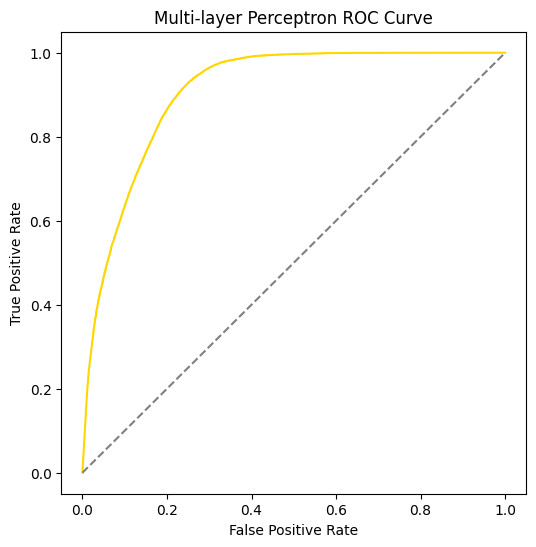
\includegraphics[width=0.5\linewidth]{MLP_perf.png}
    \caption{ROC Curve of Multi-Layer Perceptron Classifier}
    \label{fig:enter-label}
\end{figure}

\begin{table}[H]
\centering
\caption{Classification Report for MLP Classifier}
\begin{tabular}{lcccc}
\textbf{Class} & \textbf{Precision} & \textbf{Recall} & \textbf{F1-Score} & \textbf{Support} \\
-1.0 (Non-Cloud) & 0.76 & 0.93 & 0.84 & 32798 \\
1.0 (Cloud)      & 0.83 & 0.54 & 0.66 & 21244 \\
\textbf{Accuracy} & & & 0.78 & 54042 \\
\textbf{Macro Avg} & 0.80 & 0.74 & 0.75 & 54042 \\
\textbf{Weighted Avg} & 0.79 & 0.78 & 0.77 & 54042 \\
\end{tabular}
\end{table}

\subsection{Model 3: Support Vector Classifier}
Support vector machine (SVM) transforms our nonlinear data to higher dimension with kernel trick so that finding linear separation is easier. SVM can also efficiently control overfitting and adapt to handle imbalanced datasets by adjusting the hyperparameters. 

We used the same metrics here as for the random forest classifier to evaluate the performance of the model. The SVM achieves a 81.21\% accuracy and a 92.66\% ROC-AUC on the test set, proving its effectiveness in differentiating two different classes. The SVM performs better (84\% precision) on cloud pixels, but maintained reasonable performance (80\%) on non-cloud pixels. Furthermore, our model achieves a 94.4\% accuracy on cross validation set. The relatively large discrepency between training and testing accuracy may indicate our model has potential overfitting problem which can be further attenuated by more feature engineering work.
\begin{figure}[H]
    \centering
    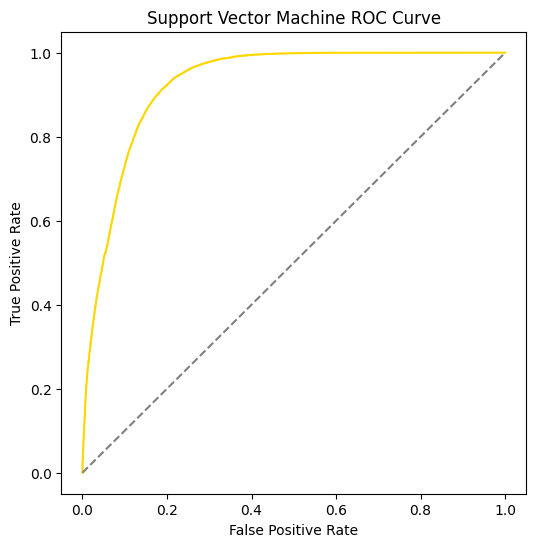
\includegraphics[width=0.5\linewidth]{SVM_per.png}
    \caption{ROC Curve of SVM Classifier}
    \label{fig:enter-label}
\end{figure}

\begin{table}[H]
\centering
\caption{Classification Report for SVM Classifier}
\begin{tabular}{lcccc}
\textbf{Class} & \textbf{Precision} & \textbf{Recall} & \textbf{F1-Score} & \textbf{Support} \\
-1.0 (Non-Cloud) & 0.80 & 0.92 & 0.86 & 32798 \\
1.0 (Cloud)      & 0.84 & 0.64 & 0.73 & 21244 \\
\textbf{Accuracy} & & & 0.81 & 54042 \\
\textbf{Macro Avg} & 0.82 & 0.78 & 0.79 & 54042 \\
\textbf{Weighted Avg} & 0.82 & 0.81  & 0.81 & 54042 \\
\end{tabular}
\end{table}



\subsection{Analysis of Convergence and Feature Importance}

We used a random forest as our 0-1 best classifier. As we can see in the Figure 10. The accuracy of the model increases with the training data, and when the training data exceeds 100,000, the rate of increase in accuracy tends to zero. The curve for the validation set follows the same trend. From both the results, it is clear that the model tends to converge when the data exceeds 100k. This indicates that the model performance increases steadily and flattens out with the number of training samples, suggesting that the model is close to convergence and does not need a large amount of new data.
\begin{figure}[H]
    \centering
    \includegraphics[width=0.5\linewidth]{learningCurve.png}
    \caption{Learning Curve for Random Forest}
    \label{fig:}
\end{figure}
We want to continue to determine if the performance of the model continues to rise as the number of decision trees increases. We constructed our random forest model sequentially from 5 to 100 trees in steps of 5 trees each and experimented on the same training and test sets using the optimal number of training and test sets obtained in the previous section. The “number of trees vs. accuracy” curve is plotted. From image 11, we can see that the training accuracy is very high and continues to improve with the increase in the number of trees, indicating that the Random Forest is able to fit the training data perfectly. The accuracy stabilizes after about 25 trees and does not increase significantly at 100 trees, indicating that the marginal benefit of adding more trees is very limited. From the above results we can conclude that 25-50 trees are sufficient to achieve almost optimal test accuracy.
\begin{figure}[H]
    \centering
    \includegraphics[width=0.5\linewidth]{AccuracyvsNumberofTreesinRandomForest.png}
    \caption{Accuracy vs Number of Trees in Random Forest}
    \label{fig:}
\end{figure}
% We then quantify and visualize the relative size of the contribution of each feature in the Random Forest model to the classification decision, using “Mean Impurity Reduction” as the metric. From the generated bar charts, it can be visualized that the MDI scores of SD, grad_feature, NDAl, and CORR. features are much higher than the other features, indicating that they contribute the most to reducing the impurity of the tree nodes and improving the classification accuracy. The remaining features (e.g., ae6, ae5 and lower ae series) have scores close to zero, indicating that their impact on the model prediction performance is almost negligible. From this result, we can consider prioritizing the key features with high MDI scores to reduce the complexity of the model and the risk of overfitting.
\begin{figure}[H]
    \centering
    \includegraphics[width=0.5\linewidth]{MDIScoreofEachFeatureInRandomForest.png}
    \caption{MDI Score of Each Feature In Random Forest}
    \label{fig:}
\end{figure}
We then use replacement importance to measure the true contribution of the above four features to the model's predictive performance. From the image below, we can see that AN and and NDA have the highest importance scores. This shows that when they are randomly disrupted, the model accuracy decreases the most, indicating that these two features are critical to the prediction results. Compared to the MDI scores in the middle above, here is a more intuitive reflection of the real impact of features on the model generalization performance.
\begin{figure}[H]
    \centering
    \includegraphics[width=0.5\linewidth]{PermutationImportance.png}
    \caption{Permutation Importance Score of Each Feature in Random Forest}
    \label{fig:}
\end{figure}
% \subsection{Post-Hoc EDA}

\subsection{Stability Check and Generalizations}

To test how stable our results were, we revised one of the key decisions we made during the feature engineering: adding the grad\_feature. This feature captures the average gradient, or local variation, in intensity around each pixel. We conjectured the feature would help the models discern between cloudy areas which could be more textured compared to smoother, non-cloudy regions -- or vice versa -- and our initial feature importance analysis confirmed our priors. However, to understand how much our models depend on this feature, we removed grad\_feature and re-ran both the Random Forest and Multi-Layer Perceptron models with everything else kept the same.


What we found was that performance dropped, but not drastically. The Random Forest model's accuracy went from around 83.7\% down to 79.3\%, and its ROC-AUC dropped by around 3.4 points. The MLP saw a similar dip as accuracy dropped by 5\%, and ROC-AUC by about 3.9 points. So, while the models still worked without the feature, it clearly added value. When we looked at the predictions visually, the models without grad\_feature tended to miss thin or faint clouds, suggesting that this kind of texture-based information really helps capture edge cases.


We also wanted to see how well our models generalize to new data. Since we only had three labeled images, we trained on two and tested on the third, rotating the test image each time. This mimics a real-world setting, where we’d be applying the model to new satellite images. Overall, performance held up pretty well. The one exception was O013257, which seemed to have different lighting or structure compared to the others, making it harder to classify. Interestingly, when we included O013257 in training instead of testing, the models generalized better, probably because it added more variety to the training set.


In the end, our models showed a good degree of stability and generalizability. They weren’t overly sensitive to one specific feature, though the grad\_feature definitely helped. And while we saw some variation in performance across images, the models were generally reliable: especially when trained on more diverse examples. That said, adding more labeled images in the future would go a long way toward making these models even more robust, especially for challenging or ambiguous scenes.

\newpage
\section{Bibliography}
Shi, T., Yu, B., Clothiaux, E. E., \& Braverman, A. J. (2008). Daytime arctic cloud detection based on multi-angle satellite data with case studies. Journal of the American Statistical Association, 103(482), 584-593.

\appendix

\section{Academic honesty}

\subsection{Statement}
We hereby affirm to Professor Bin Yu and the STAT214 staff that we will uphold the highest standards of academic integrity throughout this semester at UC Berkeley. We commit to adhering to all ethical guidelines, avoiding any form of dishonesty, and ensuring that my work reflects genuine effort and understanding.

We fully acknowledge that engaging in unethical practices, such as plagiarism, unauthorized collaboration, or misrepresentation of work, can have serious academic consequences, including potential disciplinary action or probation. Therefore, we declare that all the submitted work, including, but not limited to, code, reports, and documentation, has been primarily conceived, designed, and executed by us. Any external resources or collaborations, if applicable, will be properly credited in accordance with academic policies.

We take full responsibility for maintaining the integrity of our work and contributing to a fair and honest learning environment.
\subsection{LLM Usage}
We used LLM only to help correcting the grammars in this report.

% \subsubsection*{Coding}

% \subsubsection*{Writing}

\end{document}
    